\documentclass[oneside,13pt,a4paper]{article}

% Chargement d'extensions
\usepackage[utf8]{inputenc}
\usepackage[french]{babel}
\usepackage{graphicx}
\usepackage[top=3cm, bottom=3cm, left=3cm, right=3cm]{geometry}
\usepackage{amsmath}
\usepackage{amssymb}
\usepackage{array}
% Liens et autres
\usepackage{hyperref}
\hypersetup{
    colorlinks=true,
    linkcolor=black,
	urlcolor=blue,
	pdftitle={Rendu},
	bookmarks=true,
}

% Bout de code
\usepackage{listings}
\usepackage{color}

\definecolor{mygreen}{rgb}{0,0.6,0}
\definecolor{mygray}{rgb}{0.5,0.5,0.5}
\definecolor{mymauve}{rgb}{0.58,0,0.82}

\lstset{
  backgroundcolor=\color{white},   % choose the background color; you must add \usepackage{color} or \usepackage{xcolor}; should come as last argument
  basicstyle=\footnotesize,        % the size of the fonts that are used for the code
  breakatwhitespace=false,         % sets if automatic breaks should only happen at whitespace
  breaklines=false,                 % sets automatic line breaking
  captionpos=b,                    % sets the caption-position to bottom
  commentstyle=\color{mygreen},    % comment style
  deletekeywords={...},            % if you want to delete keywords from the given language
  escapeinside={\%*}{*)},          % if you want to add LaTeX within your code
  extendedchars=true,              % lets you use non-ASCII characters; for 8-bits encodings only, does not work with UTF-8
  firstnumber=0,                   % start line enumeration with line 1000
  frame=single,	                   % adds a frame around the code
  keepspaces=true,                 % keeps spaces in text, useful for keeping indentation of code (possibly needs columns=flexible)
  keywordstyle=\color{magenta},       % keyword style
  %language=C++,                    % the language of the code
  morekeywords={PREFIX,FILTER,UNION,WHERE,CONSTRUCT},            % if you want to add more keywords to the set
  numbers=left,                    % where to put the line-numbers; possible values are (none, left, right)
  numbersep=5pt,                   % how far the line-numbers are from the code
  numberstyle=\tiny\color{mygray}, % the style that is used for the line-numbers
  rulecolor=\color{black},         % if not set, the frame-color may be changed on line-breaks within not-black text (e.g. comments (green here))
  showspaces=false,                % show spaces everywhere adding particular underscores; it overrides 'showstringspaces'
  showstringspaces=false,          % underline spaces within strings only
  showtabs=false,                  % show tabs within strings adding particular underscores
  stepnumber=2,                    % the step between two line-numbers. If it's 1, each line will be numbered
  stringstyle=\color{mymauve},     % string literal style
  tabsize=4,	                   % sets default tabsize to 2 spaces
  literate=
  {á}{{\'a}}1 {é}{{\'e}}1 {í}{{\'i}}1 {ó}{{\'o}}1 {ú}{{\'u}}1
  {Á}{{\'A}}1 {É}{{\'E}}1 {Í}{{\'I}}1 {Ó}{{\'O}}1 {Ú}{{\'U}}1
  {à}{{\`a}}1 {è}{{\`e}}1 {ì}{{\`i}}1 {ò}{{\`o}}1 {ù}{{\`u}}1
  {À}{{\`A}}1 {È}{{\'E}}1 {Ì}{{\`I}}1 {Ò}{{\`O}}1 {Ù}{{\`U}}1
  {ä}{{\"a}}1 {ë}{{\"e}}1 {ï}{{\"i}}1 {ö}{{\"o}}1 {ü}{{\"u}}1
  {Ä}{{\"A}}1 {Ë}{{\"E}}1 {Ï}{{\"I}}1 {Ö}{{\"O}}1 {Ü}{{\"U}}1
  {â}{{\^a}}1 {ê}{{\^e}}1 {î}{{\^i}}1 {ô}{{\^o}}1 {û}{{\^u}}1
  {Â}{{\^A}}1 {Ê}{{\^E}}1 {Î}{{\^I}}1 {Ô}{{\^O}}1 {Û}{{\^U}}1
  {Ã}{{\~A}}1 {ã}{{\~a}}1 {Õ}{{\~O}}1 {õ}{{\~o}}1
  {œ}{{\oe}}1 {Œ}{{\OE}}1 {æ}{{\ae}}1 {Æ}{{\AE}}1 {ß}{{\ss}}1
  {ű}{{\H{u}}}1 {Ű}{{\H{U}}}1 {ő}{{\H{o}}}1 {Ő}{{\H{O}}}1
  {ç}{{\c c}}1 {Ç}{{\c C}}1 {ø}{{\o}}1 {å}{{\r a}}1 {Å}{{\r A}}1
  {€}{{\euro}}1 {£}{{\pounds}}1 {«}{{\guillemotleft}}1
  {»}{{\guillemotright}}1 {ñ}{{\~n}}1 {Ñ}{{\~N}}1 {¿}{{?`}}1
}

% Commande pour notation 'NB :' (nota bene)
\newcommand\nb[1][0.3]{N\kern-#1emB : }

% Espacement entre les paragraphes
\parskip=5pt

% csquotes va utiliser la langue définie dans babel
\usepackage[babel=true]{csquotes}

% pour afficher Schéma au lieu de figure dans les legende des images
\addto\captionsfrench{\def\figurename{Schéma}}

% Informations le titre, le(s) auteur(s), la date
\title{}
\author{
    Chakib ELHOUITI \and
    Massili KEZZOUL \and
    Belkassim BOUZIDI
}
\date{\today}


\begin{document}
%\maketitle
\begin{titlepage}
	\centering
	{\scshape\LARGE Universite de Montpellier\par}
	{\scshape\Large\par}
	\vspace{1.5cm}
	{\huge\bfseries Rapport de projet \\Ingénierie des Connaissances\par}
	\vspace{2cm}
	{\Large\itshape
    Belkassim BOUZIDI \\
		Chakib ELHOUITI \\
		Massili KEZZOUL \\
		\par}

		\vspace{2cm}

	\begin{figure}[h]
		\begin{minipage}[c]{.46\linewidth}
			\centering
			
\includegraphics[width=1\textwidth]{img/univ-montpellier.png}
		\end{minipage}
		\hfill%
		\begin{minipage}[c]{.46\linewidth}
			\centering
			
\includegraphics[width=1\textwidth]{img/fds.png}
		\end{minipage}
	\end{figure}

	\par\vspace{1cm}

	\vfill

	% Bottom of the page
	{\large \today\par}
\end{titlepage}

\section{Introduction}

Dans le cadre de ce projet, il est demandé, pour un domaine applicatif, de proposer une illustration de mise en œuvre des techniques et technologies de l’Ingénierie des Connaissances.

\section {Définition des objectifs d'application}

\subsection{Contexte métier et objectifs}

Le domaine applicatif choisi est le pari sportif. L'objectif est de définir une base de connaissance qui permettra de classer des matches de football en plusieurs niveaux de risques d'un point de vu d'un parieur. Afin de simplifier la modélisation et l’implémentation pour une première version, nous ne considérons ici que la \href{https://fr.wikipedia.org/wiki/Championnat_d%27Angleterre_de_football}{Premier League}, le championnat d'Angleterre de football.

À partir de cette base de connaissance, le but est d'exécuter des requêtes SPARQL et/ou DL afin de trouver les équipes pour lesquelles parier avec un risque qui doit être le plus faible possible.

Selon la précision qui découlera de l'implémentation, ce projet peut-être utilisé pour de l'aide à la décision pour de parieurs professionnels ou de simples recommandations pour des parieurs amateurs.

\subsection{Quelques scénarios d'utilisation}
\label{scenario}

Un scénario type d'utilisation est de demander, via une requête SPARQL par exemple, de trouver une relation entre une équipe et un match à venir, tel que cette équipe à de fortes chances de gagner.

Cette relation représentera donc, d'une façon, la probabilité que cette équipe gagne ce match. Cela se fera en définissant cette relation comme étant une conjonction de certains critères qui favorisent la victoire d'une équipe à un match. Voici une liste non-exhaustive de ces critères : 

\begin{itemize}
  \item Cette équipe joue à domicile;
  \item Elle a une meilleur forme que son adversaire;
  \item Elle a un meilleur classement que son adversaire dans la ligue;
  \item Et bien d'autres ...
\end{itemize}

\section{La mise en œuvre}

Après avoir défini le contexte métier ainsi que les objectifs voulus, nous avons commencé à mètre en œuvre notre ontologie.

\subsection{Modélisation}

La première étape consiste en la définition de la composante terminologique (la TBOX).

\subsubsection{Les classes et propriétés de base}

\paragraph{Team}

On a commencé par la plus évidente, une équipe de football.

\begin{tabular}{| l | l | c | c | p{3cm} |}
  \hline
  \multicolumn{5}{|c|}{Propriètes de la classe \textbf{Team}} \\ \hline
  Détail & Nom de la propriétés & Domaine & Co-domaine & Notes \\ \hline
  le nom d'une équipe & rdfs:label  & X & X &  \\ \hline
  Joue un match & PlayedAGame & Team & Game &  \\ \hline
  A un entraîneur & ManagedBy & Team  & Manager &  \\ \hline
  Classement Actuel & rank  & Team & Manager &  \\ \hline
  Nombre de victoire & nWin & Team & int &  \\ \hline
  Nombre de match Nul & nDraw & Team & int &  \\ \hline
  Nombre de défaite & nLose & Team & int &  \\ \hline
  La forme Actuel & currentFrom & Team & int & La forme est représentée par la somme des point acquis lors des 5 derniers matchs. \\ \hline
  Joue ce match à domicile & playGameHome & Team & Game & \\ \hline
  Joue ce match à l'extérieur & playGameAway & Team & Game & \\ \hline
  A gagner ce match & winner & Team & GamePlayed & \\ \hline
  A perdu ce match & looser & Team & GamePlayed & \\ \hline
  A joué contre cette équipe & playedAgainst & Team & Team & \\
  \hline
\end{tabular}

\paragraph{Manager}

Chaque équipe a un entraîneur. Le but de cette classe est de pouvoir définir quelques critères (Voir \nameref{scenario}) associés à la forme de l’entraîneur et son historique avec l’équipe qu’il va affronter.

\begin{tabular}{| l | l | c | c | p{3cm} |}
  \hline
  \multicolumn{5}{|c|}{Propriètes de la classe \textbf{Manager}} \\ \hline
  Détail & Nom de la propriétés & Domaine & Co-domaine & Notes \\ \hline
  Nom de l'entraîneur & rdfs:label & X  & X  &  \\ \hline
  Entraîne une équipe & Manage & Manager & Team &  \\
\hline
\end{tabular}

\begin{figure}[h]
  \centering
  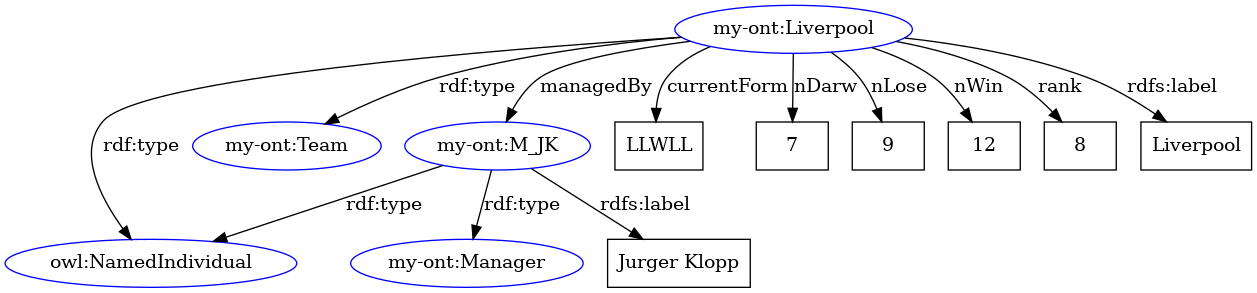
\includegraphics[width=\textwidth]{img/team.png}
  \caption{Représenation d'une équipe et son entraîneur}
\end{figure}

\paragraph{Referee}

Chaque match de football se dispute sous le contrôle d’un arbitre central, disposant de toute l’autorité nécessaire pour veiller à l’application des Lois du Jeu dans le cadre du match qu’il est appelé à diriger. Bien qu'il est tenu d'être le plus neutre possible, ils influent souvent sur la stratégie choisie par les entraîneurs.

\begin{tabular}{| l | l | c | c | p{3cm} |}
  \hline
  \multicolumn{5}{|c|}{Propriètes de la classe \textbf{Referee}} \\ \hline
  Détail & Nom de la propriétés & Domaine & Co-domaine & Notes \\ \hline
  Nom & rdfs:label  & X  &X  &  \\ \hline
  Arbitre un match & referee & Referee & Game & contraire de redereedBy  \\ \hline
  Nombre de HomeWIn & homeWin & Referee & int  & Nombre de match que l'arbitre a fait gagner à l'équipe jouant à domicile  \\ \hline
  Nombre de AwayWin & awayWin & Referee & int & Nombre de match que l'arbitre a fait gagner à l'équipe jouant à l'extérieur \\ \hline
  Nombre de matchs nuls & refereeDraw & Referee & int &  \\ 
  \hline
\end{tabular}

\nb Les propriétés \textit{homeWin}, \textit{awayWin} et \textit{refereeDraw} sont utiles pour voir si un arbitre est plutôt avantageux pour les équipes jouant à domicile ou à l’extérieur.

\paragraph{Game}

On arrive ici au cœur du problème. Il s’agit de définir un match et ses propriétés les plus utiles pour atteindre nos objectifs. On a décidé qu’il fallait différencier les matchs qui se sont déjà joués des matches qui arrivent. La classe \textit{Game} a donc deux sous-classes : \textit{GamePlayed} et \textit{GameUpComing}. Les propriétés associées à ces classes sont les suivantes :

\begin{tabular}{| l | l | c | c | p{3cm} |}
  \hline
  \multicolumn{5}{|c|}{Propriètes de la classe \textbf{Game} et ses sous-classes} \\ \hline
  Détail & Nom de la propriétés & Domaine & Co-domaine & Notes \\ \hline
  Date du match & dateGame & Game & string & … \\ \hline
  L'équipe qui joue à domicile & homeTeam  & Game & Team& \\ \hline
  L'équipe qui joue à l'extérieur & awayTeam & Game & Team& \\ \hline 
  Nombre de but domicile& fullTimeHomeGoal & GamePlayed & int & … \\ \hline
  Nombre de but extérieur& fullTimeAwayGoal & GamePlayed & int& … \\ \hline
  L'arbitre du match & refereedBy & Game & Referee & Contraire de referee \\ \hline
  Vainqueur & winner & GamePlayed & Team & Le vainqueur d'un match \\ \hline
  Perdant & looser & GamePlayed & Team & Le perdant d'un match \\
  \hline
\end{tabular}

\begin{figure}[!h]
  \centering
  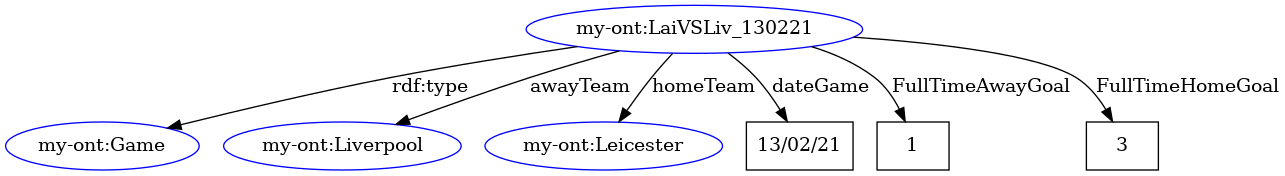
\includegraphics[width=0.96\textwidth]{img/game.png}
  \caption{Représenation d'un match et son arbitre}
\end{figure}

\subsubsection{Les propriétés inférées}

Certaines des ces propriétés ne sont pas à définir explicitement dans la \textbf{ABOX}, car elles seront inférées automatiquement par le raisonneur de Protégé ou déduites par des requêtes SPARQL.

\paragraph{manager et managedBy}

\textit{manager} et \textit{managedBy} sont un exemple des propriétés inférées par le raisonneur. En effet, il suffit d'ajouter à la \textbf{ABOX} que M \textit{manage} T alors il déduira automatiquement que T \textit{managedBy} M.

\paragraph{winner et looser}

Le cas de \textit{winner} et \textit{looser} est plus particulier. Pour qu’une équipe soit la vainqueur d’un match alors elle doit participer à ce match et marquer plus de buts que son adversaire. Donc on peut l’écrire de cette façon :

\begin{multline*}
winner(g,t) \equiv \exists a,\exists h  fullTimeHomeGoal(g,h) \ \wedge \ fullTimeAwayGoal(g, a) \ \wedge \ \\
  (homeTeam(g,t) \ \wedge \ h > a)  \vee (awayTeam(g,t) \ \wedge \  a > h) \\
\end{multline*}

Mais ce genre d'équivalence ne peut être déduite par le raisonneur de Protégé. Pour remédier à cela nous avons écrit une requête SPARQL pour déduire automatiquement ces relations.

\lstinputlisting[caption=Requête qui déduit les propriétés \textit{winner} et \textit{looser}]{../ontologies/sparql-construct/winner-looser.sql}

\subsubsection{Les contraintes favorisent la victoire}

L'idée générale est de déduire des relations, entre une équipe et un match à venir, qui indiques que cette équipe a des chances de gagner ce match. Pour cela, on définit les propriétés suivantes : 

\begin{tabular}{| p{5cm} | l | c | c |}
  \hline
  Détail & Nom de la propriétés & Domaine & Co-domaine\\ \hline
  l'équipe a de forte chances de gagner ce match & highProb & Team & GameUpComing  \\ \hline
  l'équipe a des chances de gagner ce match & medProb & Team & GameUpComing  \\ \hline
  l'équipe a peu de chances de gagner ce match & lowProb & Team & GameUpComing  \\
  \hline
\end{tabular}

Avant de définir concrétement ces propriétés, on doit d'abord définir les facteurs qui favorisent la victoire d'une équipe.

\paragraph{Contraintes de base}

Elles prendront la forme d’une propriété dont le domaine est \textit{Team}.

\begin{tabular}{| p{5cm} | l | c | c |}
  \hline
  Détail & Nom de la propriétés & Domaine & Co-domaine\\ \hline
  L'équipe joue à domicile & playGameHome & Team & Game  \\ \hline
  L'équipe a un meilleur classement que son adversaire & bestRankThan & Team & Team  \\ \hline
  Le classement de l'équipe est largement mieux que son adversaire & best10RankThan & Team & Team \\ \hline
  l'équipe a une meilleur forme que son adversaire & bestFormThan & Team & Team  \\
  \hline
\end{tabular}

\paragraph{Généralisation des contraintes} Une fois les contraintes de base définit et afin de simplifier la définition des relations finales, nous passons par cette étape de généralisation des contraintes de base. Cela consiste en la transformation des propriétés précédemment définies en propriétés qui ont toutes comme domaine \textit{Team} et comme co-domaine \textit{GameUpComing}.

Par exemple, la propriété \textit{Team} \textit{bestRankThan} \textit{Team} va devenir \textit{Team} \textit{c2} \textit{GameUpComing}. La sémantique associée à \textit{c2} sera : \guillemotleft une équipe a un meilleur classement que l'équipe contre laquelle elle va jouer à ce match.\guillemotright

\lstinputlisting[firstline=7,lastline=20,caption=Requête qui transforme \textit{bestRankThan} en \textit{c2}]{../ontologies/sparql-generalization/c2.sql}

On aura donc ce qui suit :
\begin{description}
  \item[c1] associée a \textit{playGameHome}
  \item[c2] associée a \textit{bestRankThan}
  \item[c3] associée a \textit{best10RankThan}
  \item[c4] associée a \textit{bestFormThan}
\end{description}

\paragraph{Conjonctions des contraintes}

Enfin, les propriétés finales ne seront que des conjonctions des contraintes généralisées.

\begin{description}
  \item[highProb] est définie comme étant la conjonction de toutes les contraintes. 
  \[highProb(t,g) \equiv c_1(t,g) \wedge c_2(t,g) \wedge c_3(t,g) \wedge c_4(t,g)\]
  \item[medProb] est définie comme étant la conjonction de 2 ou 3 contraintes.
  \item[lowProb] est définie comme étant le conjonction d'une seule contrainte.
\end{description}

\subsection{Constitution de la ABOX}

Une fois la \textbf{TBOX} définie et construite, nous devons récupérer les assertions qui constitueront les faits de notre \textbf{ABOX}. Pour cela, nous avons extrait, via un script python\footnote{Vous trouverez le script ici : \href{../db/update.py}{update.py}}, les matches qui se sont déroulés à ce jour\footnote{\url{https://www.football-data.co.uk/mmz4281/2021/E0.csv}} ainsi que le classement actuel\footnote{\url{https://www.msn.com/en-au/sport/football/epl/ladder}} de la \textit{Premier league}.

À ce stade, nous avons donc toutes les informations dont on a besoin sous un format CSV. On a ensuite définis des scripts python, à l'aide de la librairie \href{https://github.com/RDFLib/rdflib}{RDFLib}, afin de générer les faits constituant la \textbf{ABOX}.

Il faut noter que, à ce stade, les faits ne contiennent que certaines propriétés de base. Le reste sera inférées par un raisonneur et des requêtes SPARQL.

\subsection{Autres composants}

(enrichissement de la base, raisonneur, Triple store, API de programmation)

Afin de générer toutes les propriété dont on a besoin, nous fesont appele à plusieurs programmes.

\subsubsection{Raisonneur}



\subsubsection{Requêtes SPARQL}


\section{Illustration d'utilisation}

en réponse aux objectifs fixés (e.g. requête SPARQL
et/ou DL, exemples de classification automatique).

\section{Résultat et perspectives}

\subsection{Résultat}

Une discussion sur le résultat obtenu en présentant les perspectives envisageables

\subsection{Perspectives}

(e.g. couplage avec des vocabulaires externes)

\subsection{Avantages et limites de l’Ingénierie des Connaissances}

rencontrés lors de la réalisation de votre projet.

\section{Intérêt des ontologies par rapport aux bases de données relationnelles}

Important : une discussion sur l’intérêt des ontologies par rapport aux bases de données de
type SGBDR/BD No SQL (2 à 3 pages).

\end{document}
